\section{Optimización mediante PPO y GRPO}
\label{sec:marco-optimizacion}
La recompensa orienta la actualización de la política al favorecer las respuestas mejor evaluadas, mientras que PPO y GRPO incorporan mecanismos para controlar esos cambios.

\subsection{Ciclo de optimización y mecanismos de estabilidad}
\label{sec:ciclo-optimizacion}
El ciclo de entrenamiento comienza al seleccionar consultas y generar respuestas mediante una política de muestreo, a partir de las cuales se calculan recompensas y ventajas para actualizar los parámetros. La ventaja indica qué tan favorable resulta una acción o respuesta respecto de una referencia de comparación, lo que permite distinguir una recompensa alta en términos absolutos de una respuesta mejor que las alternativas consideradas. Después de la actualización, se vuelve a generar con la política modificada y se repite el procedimiento, como se representa en la figura \ref{fig:ciclo-rl}~\cite{schulman2017ppo,shao2024deepseekmath}.

\begin{figure}[htbp]
\centering
\begingroup
\singlespacing
\begin{tikzpicture}[>=Stealth,
 box/.style={draw,rounded corners=2pt,align=center,text width=3.2cm,minimum height=1.1cm,font=\small},
 lbl/.style={font=\small,align=center}]
\node[box] (q) at (0,0) {Consultas del conjunto de entrenamiento};
\node[box] (p) at (4.5,0) {Política de recolección\\Generación de respuestas};
\node[box] (e) at (9,0) {Evaluador externo\\Cálculo de recompensas};
\node[box] (u) at (0,-2.5) {Política actual\\Actualización de parámetros};
\node[box] (a) at (4.5,-2.5) {Ventajas y probabilidades de los tokens};
\node[box,dashed] (ref) at (9,-2.5) {Política de referencia\\Comparación mediante KL};
\draw[->] (q)--(p); \draw[->] (p)--(e);
\draw[->] (e.south)--(9,-1.25)-|(a.north east);
\draw[->] (p.south)--(a.north);
\draw[->] (a)--(u);
\draw[->,dashed] (ref.south)--++(0,-0.6)-|(u.south);
\draw[->] (u.west)--(-2.2,-2.5)--(-2.2,1.35)--(4.5,1.35)--(p.north);
\node[lbl] at (4.1,1.95) {La política actualizada se usa en la siguiente iteración};
\end{tikzpicture}
\endgroup

\caption{Ciclo de generación, evaluación y actualización de la política.}
\label{fig:ciclo-rl}
\end{figure}

Para interpretar este ciclo conviene distinguir la política actual $\pi_\theta$, cuyos parámetros se optimizan, de la política de recolección $\pi_{\mathrm{old}}$, utilizada para generar el conjunto de respuestas de una iteración. Mientras se realizan actualizaciones sobre ese conjunto, ambas pueden diferir, por lo que el algoritmo compara las probabilidades de los tokens bajo las dos políticas. Por otra parte, la política de referencia $\pi_{\mathrm{ref}}$ puede mantenerse fija para regularizar la distancia respecto de un comportamiento inicial, y no debe confundirse con la política que produjo las respuestas de la iteración~\cite{shao2024deepseekmath}.

El muestreo permite obtener distintas respuestas para una misma consulta y, por ello, influye en las alternativas que el entrenamiento puede explorar. Sin embargo, aumentar la diversidad no garantiza que las respuestas sean útiles, mientras que una generación completamente determinista puede reducir la variación necesaria para comparar alternativas. Para controlar la actualización, algunos métodos utilizan clipping sobre la razón de probabilidades y una penalización por divergencia de Kullback y Leibler (KL). El primero limita el incentivo del objetivo a ciertos cambios respecto de la política de recolección, mientras que la segunda penaliza la distancia respecto de una política de referencia, por lo que cumplen funciones distintas y ninguno garantiza por sí solo la estabilidad del entrenamiento~\cite{schulman2017ppo,ouyang2022instructgpt}.

Para un estado fijo $s$, la divergencia KL entre la política actual y la de referencia se define como
\begin{equation}
D_{\mathrm{KL}}\!\left(\pi_\theta(\cdot\mid s)\,\|\,\pi_{\mathrm{ref}}(\cdot\mid s)\right)
=\sum_{a\in\mathcal{V}}\pi_\theta(a\mid s)
\log\frac{\pi_\theta(a\mid s)}{\pi_{\mathrm{ref}}(a\mid s)},
\label{eq:kl}
\end{equation}
donde $\mathcal{V}$ es el vocabulario de tokens y se supone que la política de referencia asigna probabilidad positiva a las acciones consideradas. Esta divergencia compara distribuciones completas y vale cero cuando coinciden, mientras que un coeficiente $\beta$ controla su contribución al objetivo. En implementaciones de entrenamiento puede estimarse mediante los tokens muestreados, por lo que también debe documentarse el estimador utilizado, además del valor de $\beta$~\cite{shao2024deepseekmath}.

%
\subsection{PPO como antecedente de la optimización de modelos de lenguaje}
\label{sec:ppo}
Proximal Policy Optimization (PPO) pertenece a los métodos de optimización de políticas y, en su formulación habitual de actor y crítico, combina una política que selecciona acciones con una función de valor que estima el retorno esperado desde un estado. Esta estimación ayuda a calcular las ventajas utilizadas para actualizar la política, mientras que el crítico se entrena a partir de los retornos observados. Para evitar que la reutilización de las muestras incentive cambios excesivos, una variante de PPO utiliza el objetivo con clipping~\cite{schulman2017ppo},
\begin{equation}
L^{\mathrm{clip}}(\theta)=\mathbb{E}_{t}\!\left[
\min\left(\rho_t(\theta)\widehat{A}_t,
\operatorname{clip}(\rho_t(\theta),1-\epsilon_c,1+\epsilon_c)\widehat{A}_t\right)
\right],
\label{eq:ppo}
\end{equation}
donde $\rho_t(\theta)=\pi_\theta(a_t\mid s_t)/\pi_{\mathrm{old}}(a_t\mid s_t)$ compara la probabilidad de la acción observada, $\widehat{A}_t$ es su ventaja estimada y $\epsilon_c$ determina el intervalo de recorte. De este modo, cuando el cambio de probabilidad ya favorece suficientemente una acción con ventaja positiva, el objetivo deja de premiar su aumento en la rama recortada, con un comportamiento análogo para acciones con ventaja negativa. Este mecanismo no impone una cota estricta a cada cambio de parámetros, sino que modifica el incentivo de optimización.

En InstructGPT, PPO se utilizó después del ajuste supervisado para optimizar las respuestas según un modelo de recompensa aprendido de preferencias humanas, incorporando además una regularización respecto de una política de referencia~\cite{ouyang2022instructgpt}. Su aplicación requiere obtener recompensas y estimaciones de valor, lo que añade cómputo y memoria al entrenamiento, aunque la cantidad de modelos almacenados y la posibilidad de compartir componentes dependen de la implementación. Este costo motivó alternativas como GRPO, que reemplaza el crítico aprendido por una comparación de recompensas dentro de cada grupo~\cite{shao2024deepseekmath}.

En este punto, conviene distinguir el algoritmo que actualiza la política del procedimiento que asigna la recompensa, ya que tanto PPO como GRPO pueden utilizar distintas señales de evaluación. Por lo tanto, el carácter verificable de RLVR depende de cómo se comprueba la respuesta y se obtiene esa señal, mientras que la diferencia entre ambos algoritmos reside aquí en cómo estiman las ventajas para orientar la actualización~\cite{schulman2017ppo,shao2024deepseekmath,deepseek2025r1}.
%
\subsection{GRPO y la optimización relativa por grupos}
\label{sec:grpo}
Group Relative Policy Optimization (GRPO) genera varias respuestas para una misma consulta y utiliza sus recompensas para estimar una ventaja relativa, evitando entrenar un crítico separado. Si el grupo contiene $G$ respuestas con recompensas $r_1,\ldots,r_G$, una expresión simplificada de esa ventaja es
\begin{equation}
A_i=\frac{r_i-\overline{r}}{\sigma_r+\varepsilon_n},
\qquad \overline{r}=\frac{1}{G}\sum_{i=1}^{G}r_i,
\qquad \sigma_r=\sqrt{\frac{1}{G}\sum_{i=1}^{G}(r_i-\overline{r})^2},
\label{eq:ventaja-grpo}
\end{equation}
donde $\overline{r}$ representa el promedio del grupo, $\sigma_r$ su dispersión y $\varepsilon_n$ un término pequeño de estabilidad numérica. La normalización por la media y la desviación estándar corresponde al mecanismo de la formulación original, mientras que el término añadido y la convención para calcular la desviación pueden variar entre implementaciones~\cite{shao2024deepseekmath}.

Una ventaja positiva favorece un aumento de la probabilidad de la respuesta respecto de la política de recolección, mientras que una negativa produce el incentivo contrario, sujeto al objetivo con clipping y a la regularización utilizada. Por lo tanto, importa la diferencia entre las recompensas y no solamente su promedio, ya que un grupo con recompensas idénticas tiene ventajas relativas nulas bajo la ecuación \ref{eq:ventaja-grpo}, aunque puedan existir gradientes de otros términos del objetivo. La figura \ref{fig:grpo-ejemplo} ilustra este cálculo con cuatro respuestas y valores elegidos únicamente para explicar el procedimiento.

\begin{figure}[htbp]
\centering
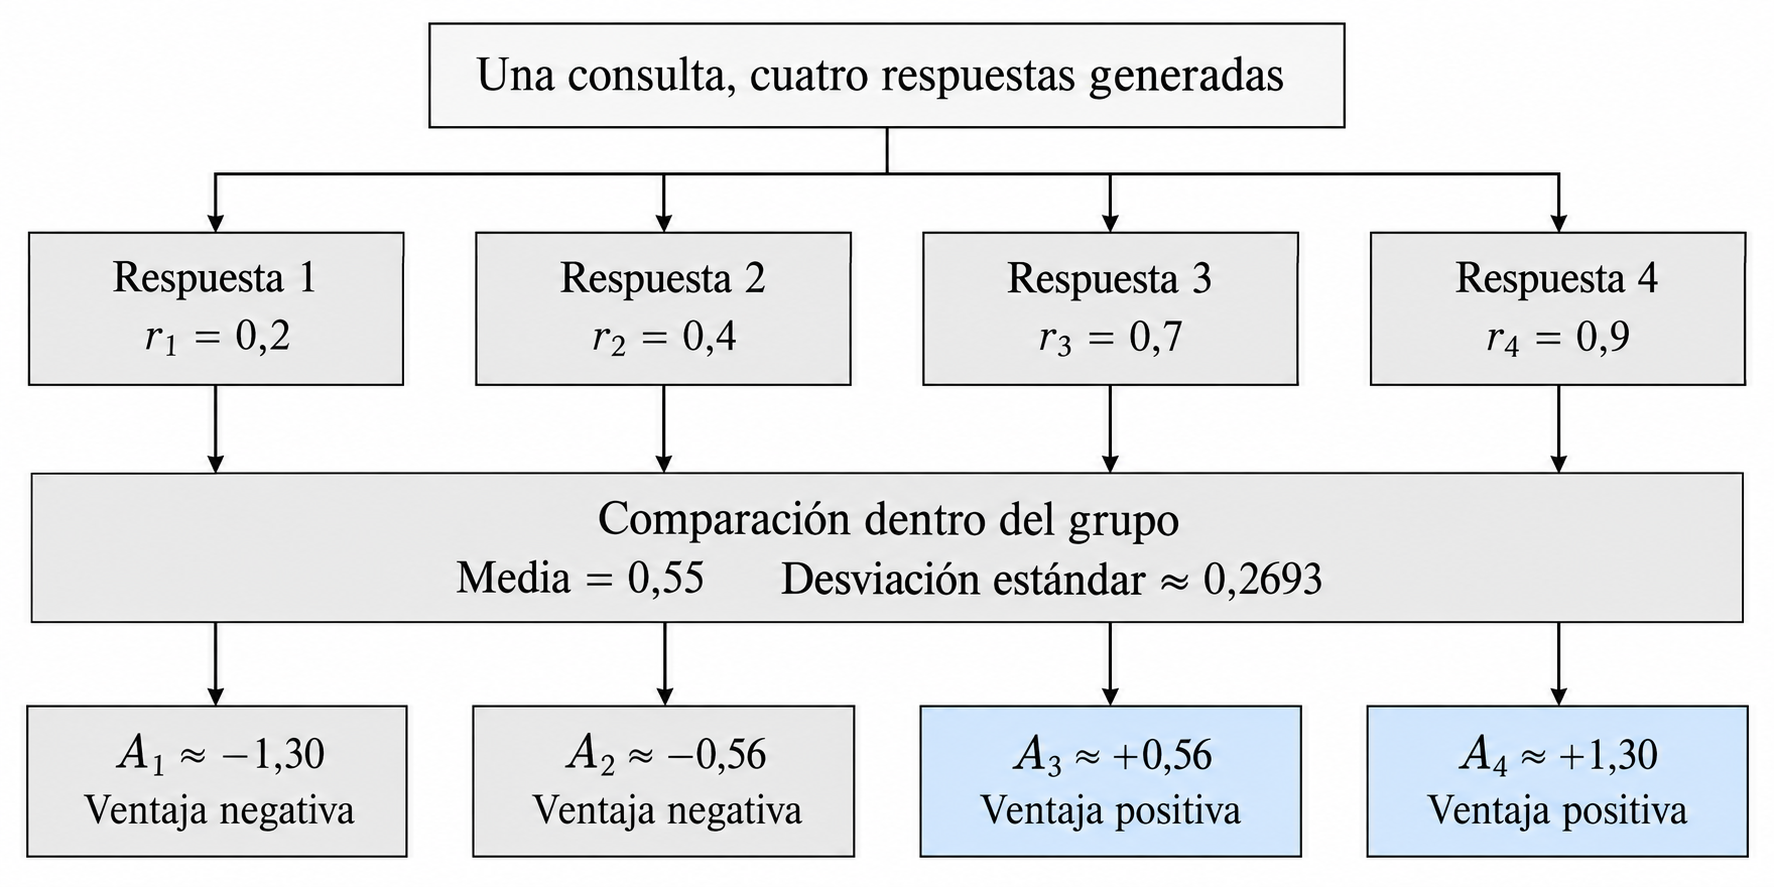
\includegraphics[width=0.95\textwidth]{Figuras/02-marco-teorico/04-ppo-grpo/rl-grpo-grupo.png}
\caption{Ejemplo ilustrativo de comparación de recompensas y ventajas en GRPO.}
\label{fig:grpo-ejemplo}
\end{figure}

Para relacionar esa comparación con la actualización de parámetros, puede escribirse el objetivo de GRPO con recompensa final como
\begin{equation}
\begin{aligned}
J_{\mathrm{GRPO}}(\theta)
&=\mathbb{E}_{x,\{y_i\}\sim\pi_{\mathrm{old}}}\left[
\frac{1}{G}\sum_{i=1}^{G}\frac{1}{T_i}\sum_{t=1}^{T_i}
\left(C_{i,t}(\theta)-\beta D_{i,t}(\theta)\right)\right],\\
C_{i,t}(\theta)
&=\min\left(\rho_{i,t}(\theta)A_i,
\operatorname{clip}(\rho_{i,t}(\theta),1-\epsilon_c,1+\epsilon_c)A_i\right),\\
\rho_{i,t}(\theta)
&=\frac{\pi_\theta(y_{i,t}\mid x,y_{i,<t})}
{\pi_{\mathrm{old}}(y_{i,t}\mid x,y_{i,<t})}.
\end{aligned}
\label{eq:objetivo-grpo}
\end{equation}
En esta expresión, las consultas se extraen de $\mathcal{D}$ y las respuestas se generan con la política de recolección, mientras que $T_i$ es la longitud de la respuesta $i$ y $D_{i,t}$ representa la divergencia respecto de la política de referencia en el contexto del token $t$. El término $C_{i,t}$ combina la razón de probabilidades con la ventaja y el recorte de PPO, mientras que $\beta D_{i,t}$ penaliza la desviación respecto de la referencia~\cite{shao2024deepseekmath}. Por lo tanto, maximizar este objetivo favorece los tokens de respuestas con mejor recompensa relativa, sujeto a esos mecanismos de control, y la pérdida utilizada para minimizar mediante descenso de gradiente puede definirse como $\mathcal{L}_{\mathrm{GRPO}}=-J_{\mathrm{GRPO}}$. La división por $T_i$ da el mismo peso total a cada respuesta antes de promediar el grupo, una elección que puede cambiar en otras variantes.

Cuando se utiliza una recompensa final, la ventaja de la respuesta puede aplicarse a sus tokens durante la actualización, aunque la formulación también contempla señales de proceso y variantes posteriores modifican la normalización y la ponderación por longitud~\cite{shao2024deepseekmath,deepseek2025r1}. En consecuencia, documentar que se utilizó GRPO no basta para reproducir una corrida, sino que deben precisarse su variante, la recompensa y las decisiones de implementación. Además, $G$ indica cuántas respuestas se generan por consulta y debe distinguirse del tamaño del microbatch y de la acumulación de gradientes, definidos en la sección \ref{sec:sft-actualizacion}.

%
